Before we dive into the physics, we take a moment to lay out some technical details, common conventions, and acronyms used throughout this note. This is intended to help the reader through the interpretation of the note.
%\addcontentsline{toc}{Section}{echnical Overview on the Content of this Note}
\subsection{Samples}
\par This analysis attempts to use all of the the latest available data and simulation samples for the MicroBooNE LEE analysis. This section briefly describes which samples are used.
\par MicroBooNE's collected data set passing  data-quality requirements for the LEE analysis consists of 10.1E20 POT of BNB data taken over four ``runs'', or data taking periods. %This number takes into account run periods discarded due to data-quality requirements. 
Only a small subset of this data is available for analyzers to use, i.e. :
\begin{itemize}
\item[-] Open on-beam data (\textbf{BNB}):
\begin{itemize}
\item ``5E19'' POT Run 1 open data set (4.54E19 POT after quality cuts)  \newline \texttt{data\_bnb\_mcc9.1\_v08\_00\_00\_25\_reco2\_C1\_beam\_good\_reco2\_5e19}
\item  ``1E19'' POT Run 3 open data set  (9.43E18 POT after quality cuts) \newline \texttt{data\_bnb\_mcc9.1\_v08\_00\_00\_25\_reco2\_G1\_beam\_good\_reco2\_1e19}
\end{itemize}
\item[-] Off-beam data (\textbf{EXT}):
\begin{itemize}
\item all available Run 1 samples (about 6.54e7 million triggers) \newline
\texttt{data\_extbnb\_mcc9.1\_v08\_00\_00\_25\_reco2\_C1\_all\_reco2} \newline
\texttt{data\_extbnb\_mcc9.1\_v08\_00\_00\_25\_reco2\_C2\_all\_reco2} \newline
\item all available Run 2 samples (about 1.52e8 million triggers) \newline 
\texttt{data\_extbnb\_mcc9.1\_v08\_00\_00\_25\_reco2\_D1\_all\_reco2} \newline
\texttt{data\_extbnb\_mcc9.1\_v08\_00\_00\_25\_reco2\_D2\_all\_reco2} \newline
\texttt{data\_extbnb\_mcc9.1\_v08\_00\_00\_25\_reco2\_E1\_all\_reco2} \newline
\texttt{data\_extbnb\_mcc9.1\_v08\_00\_00\_25\_reco2\_E2\_all\_reco2} \newline
\item all available Run 3 samples (about 2.14e8 million triggers) \newline
\texttt{data\_extbnb\_mcc9.1\_v08\_00\_00\_25\_reco2\_F\_all\_reco2} \newline 
\texttt{data\_extbnb\_mcc9.1\_v08\_00\_00\_25\_reco2\_G1\_all\_reco2} \newline
\texttt{data\_extbnb\_mcc9.1\_v08\_00\_00\_25\_reco2\_G2\_all\_reco2} \newline
\texttt{data\_extbnb\_mcc9.1\_v08\_00\_00\_25\_reco2\_G2a\_all\_reco2} \newline
\item about 250k events of NuMI off-beam data (used for BDT training only)
\newline
\texttt{numi\_uboone\_run1\_beamoff\_offset1\_mcc9\_reco2\_v08\_00\_00\_28\_v0}
\end{itemize}
\item[-] MC (from the ``overlay datasets''):
\begin{itemize}
\item 3.64E21 POT standard MC BNB flux prediction (overlay Run 1, 2, and 3) \newline
\texttt{prodgenie\_bnb\_nu\_uboone\_overlay\_mcc9.1\_v08\_00\_00\_26\_filter\_run1\_reco2\_reco2} \newline
\texttt{prodgenie\_bnb\_nu\_uboone\_overlay\_mcc9.1\_v08\_00\_00\_26\_filter\_run2\_reco2\_D1D2\_reco2} \newline
\texttt{prodgenie\_bnb\_nu\_uboone\_overlay\_mcc9.1\_v08\_00\_00\_26\_filter\_run3\_reco2\_G\_reco2} \newline
\item 1.94E23 POT $\nu_e$ intrinsic only from the standard MicroBooNE flux prediction (overlay Run 1, 2, and 3) \newline
\texttt{prodgenie\_bnb\_intrinsice\_nue\_uboone\_overlay\_mcc9.1\_v08\_00\_00\_26\_run1\_reco2\_reco2} \newline
\texttt{prodgenie\_bnb\_intrinsic\_nue\_overlay\_run2\_v08\_00\_00\_35\_run2a\_reco2\_reco2} \newline
\texttt{prodgenie\_bnb\_intrinsice\_nue\_uboone\_overlay\_mcc9.1\_v08\_00\_00\_26\_run3\_reco2\_reco2} \newline
\item 6.42E20 POT  \emph{dirt} interactions (neutrinos which interact outside of the cryostat) (overlay Run 1 and 3) \newline
\texttt{prodgenie\_bnb\_dirt\_overlay\_mcc9.1\_v08\_00\_00\_26\_run1\_reco2\_reco2} \newline
\texttt{prodgenie\_bnb\_intrinsice\_nue\_uboone\_overlay\_mcc9.1\_v08\_00\_00\_26\_run3\_reco2\_reco2} \newline
\item 4.92 and 9.85 E21 POT truth-filtered for CC and NC $\pi^0$ respectively (overlay Run 1 and 3). \newline
\texttt{prodgenie\_nc\_pi0\_uboone\_overlay-v08\_00\_00\_26\_run1\_reco2\_reco2}\newline
\texttt{prodgenie\_nc\_pi0\_uboone\_overlay\_mcc9.1\_v08\_00\_00\_26\_run3\_G\_reco2}\newline
\texttt{prodgenie\_cc\_pi0\_uboone\_overlay\_v08\_00\_00\_26\_run1\_reco2}\newline
\texttt{prodgenie\_cc\_pi0\_uboone\_overlay\_v08\_00\_00\_26\_run3\_G\_reco2}\newline
\item 1-2E22 POT of truth-filtered $\nu_{\mu}$ no $\pi^0$ samples used to enhance specific background categories which suffer from low-stats in final MC selection (see~\cite{bib:truthfilters} for further details). \newline
\texttt{prodgenie\_ncnopi\_overlay\_mcc9\_v08\_00\_00\_33\_new\_run3\_reco2\_reco2}\newline
\texttt{prodgenie\_NCcPiNoPi0\_overlay\_mcc9\_v08\_00\_00\_33\_New\_run3\_reco2\_reco2}\newline
\texttt{prodgenie\_CCmuNoPi\_overlay\_mcc9\_v08\_00\_00\_33\_all\_run3\_reco2\_reco2}\newline
\texttt{prodgenie\_filter\_CCmuCPiNoPi0\_overlay\_mcc9\_v08\_00\_00\_33\_run3\_reco2\_reco2}\newline
\texttt{prodgenie\_ncnopi\_overlay\_mcc9\_v08\_00\_00\_33\_run1\_reco2\_reco2}\newline
\texttt{prodgenie\_NCcPiNoPi0\_overlay\_mcc9\_v08\_00\_00\_33\_run1\_reco2\_reco2}\newline
\texttt{prodgenie\_CCmuNoPi\_overlay\_mcc9\_v08\_00\_00\_33\_all\_run1\_reco2\_reco2}\newline
\texttt{prodgenie\_filter\_CCmuCPiNoPi0\_overlay\_mcc9\_v08\_00\_00\_33\_run1\_reco2\_reco2}
\end{itemize}
\end{itemize}

%For on-beam data, three samples are used in this note: the ``5E19'' Run1 open dataset ($4.07E19$ POT after quality cuts), the ``1E19'' ($0.8E19$ POT after quality cuts) open Run3 data, and the $\sim3.0E20$ POT of filtered $\pi^0$ data from runs 1 and 3. 
%For off-beam data, this analysis uses all available samples from Run1 and Run3, consisting of roughly 1 million events for each run. 

The scaling factors for the Run 1, 2, and 3 combined EXT data set to match the full 6.95E20 POT is $\times0.375$, bringing the ratio of off-beam to on-beam data to $\sim$3-to-1. %Section~\ref{sec:systematics:stat} describes how statistical errors for bins with 0 EXT events are accounted for in the analysis'  sensitivity calculation. 
\par Because the various truth-filtered samples (CC $\pi^0$, NC $\pi^0$, CC 0$\pi$, NC 0$\pi$, CC n$\pi^{+/-}$0$\pi^0$, NC n$\pi^{+/-}$0$\pi^0$) contain events already simulated in the generic BNB flux, but with higher statistics, when merging MC samples in the analysis we take care to remove the events from the generic BNB MC that are present in these higher-statistics samples and POT-weight the special high-statistic samples appropriately. 

\subsection{Analysis Code}
\par This analysis uses as input ``reco2'' files produced by the MicroBooNE production team and performs three successive data-analysis steps. The code-base for each is documented in this section.
\par \textbf{NTuple production} NTuples which save the necessary reconstruction and truth information needed to perform the analysis are produced with custom analysis code integrated into \texttt{uboonecode}'s \texttt{ubana} repository in the \texttt{searchingfornues} subfolder. This code is maintained in the github repository \url{https://github.com/ubneutrinos/searchingfornues}. The branch \texttt{v30genie} is used for all NTuple production. Reco2 files are processed with the fhicl-files below:
\begin{itemize}
    \item \texttt{run\_neutrinoselectionfilter\_run1\_overlay\_cc0pinp.fcl} for Run1 and Run2 MC.
    \item \texttt{run\_neutrinoselectionfilter\_run1\_data\_cc0pinp.fcl} for Run1 data.
    \item \texttt{run\_neutrinoselectionfilter\_run3\_overlay\_cc0pinp.fcl} for Run3 MC.
    \item \texttt{run\_neutrinoselectionfilter\_run3\_dataON\_cc0pinp.fcl} for on-beam Run3 data.
    \item \texttt{run\_neutrinoselectionfilter\_run3\_dataOFF\_cc0pinp.fcl} for off-beam Run3 data.
\end{itemize}
The material presented in this tech-note was processed from tags \texttt{v08\_00\_00\_43} (MC / open-data) and \texttt{v08\_00\_00\_44} (detector systematics) of the \texttt{geniev30} branch of \texttt{searchingfornues} repository. $\nu_{\mu}$ NTuples and $\nu_e$ far-sideband NTuples were processed directly by the production team with tags \texttt{v08\_00\_00\_41} and \texttt{v08\_00\_00\_42} of \texttt{uboonecode} respectively.
\par \textbf{Plotting} Plotting code used to load input NTuples, perform event selections, calculate systematic uncertainties, and correctly POT scale distributions for MC and data/MC comparisons is available in the \texttt{PELEE} repository: \url{https://github.com/ubneutrinos/PELEE}.
\par \textbf{Sensitivity calculations} The SBNFit framework is used to extract full covariance matrices for analysis selections, assess analysis systematics, exercise the $\nu_{\mu}$ constraint and assess the analysis' sensitivity \cite{bib:sbnfitgit}.

\subsection{How to read plots in this note} A large fraction of plots in this note are data-simulation comparisons. This paragraph describes common features of these plots. An example data-MC comparison from the analysis' two-shower sideband is shown in figure~\ref{fig:exampleplot} to help orient the reader as different features are described. All plots, unless otherwise labeled, are POT normalized, following the procedure outlined in DocDB 15204~\cite{bib:POTscaling} with the POT labeled on the top-right corner. Data-simulation comparisons are accompanied by a legend which denotes the various event categories shown. Categories are described below:
\begin{itemize}
    \item \textbf{BNB}: On-beam contributions (data).
    \item \textbf{EXT}: Off-beam contributions (data).
    \item \textbf{Cosmic}: Events from MC overlay where a cosmic instead of a neutrino interaction has been selected as the neutrino candidate by Pandora's \texttt{NeutrinoID}. In this case at least $80\%$ of the hits in the neutrino slice come from overlay cosmics, instead of the true neutrino interaction. 
    \item \textbf{Out. fid. vol.}: Events from MC overlay where a neutrino was tagged, but the neutrino interaction vertex is outside of the defined TPC fiducial volume.
    \item \textbf{MiniBooNE LEE}: Events from the MB-$\nu_e$ LEE model.
    \item \textbf{$\nu_e$}: CC $\nu_e$ events, split by final state (\zpsel, \npsel, and X$\pi$, where N$\geq$1 and X$\geq$0).
    \item \textbf{$\nu_{\mu}$ CC}: CC muon events with no final state $\pi^0$.
    \item \textbf{$\pi^0$}: $\nu_{\mu}$ events with final state $\pi^0$ split into NC and CC channels.
    \item \textbf{NC}: NC events (all flavors) with no final state $\pi^0$s.
\end{itemize}{}

Error bars for data-points are computed as $\sqrt{N}$ with $N$ the number of entries in a bin\footnote{We can also produce plots with asymmetric statistical uncertainties as discussed in Appendix~\ref{app:dataerrorbars}, but these are not used by default in the note}. Error bands, when included, are shown as a semi-transparent gray band on the MC + EXT stacked entries. The shaded error-bands always include MC statistical errors, generally include flux, cross-section, and re-interaction uncertainties, and when explicitly labeled include detector systematics as well. The same convention is used for stacked data/MC comparisons as well as ratio plots. Finally, the title of each plot contains information on the selection applied or sideband of origin for the comparison, and the second row, when present, indicates what type of $\pi^0$ scaling has been applied (i.e. \texttt{$\pi^0$ scaling: [1-0.40 $\times E_{\pi}$}).


\begin{figure}[ht]
\begin{center}
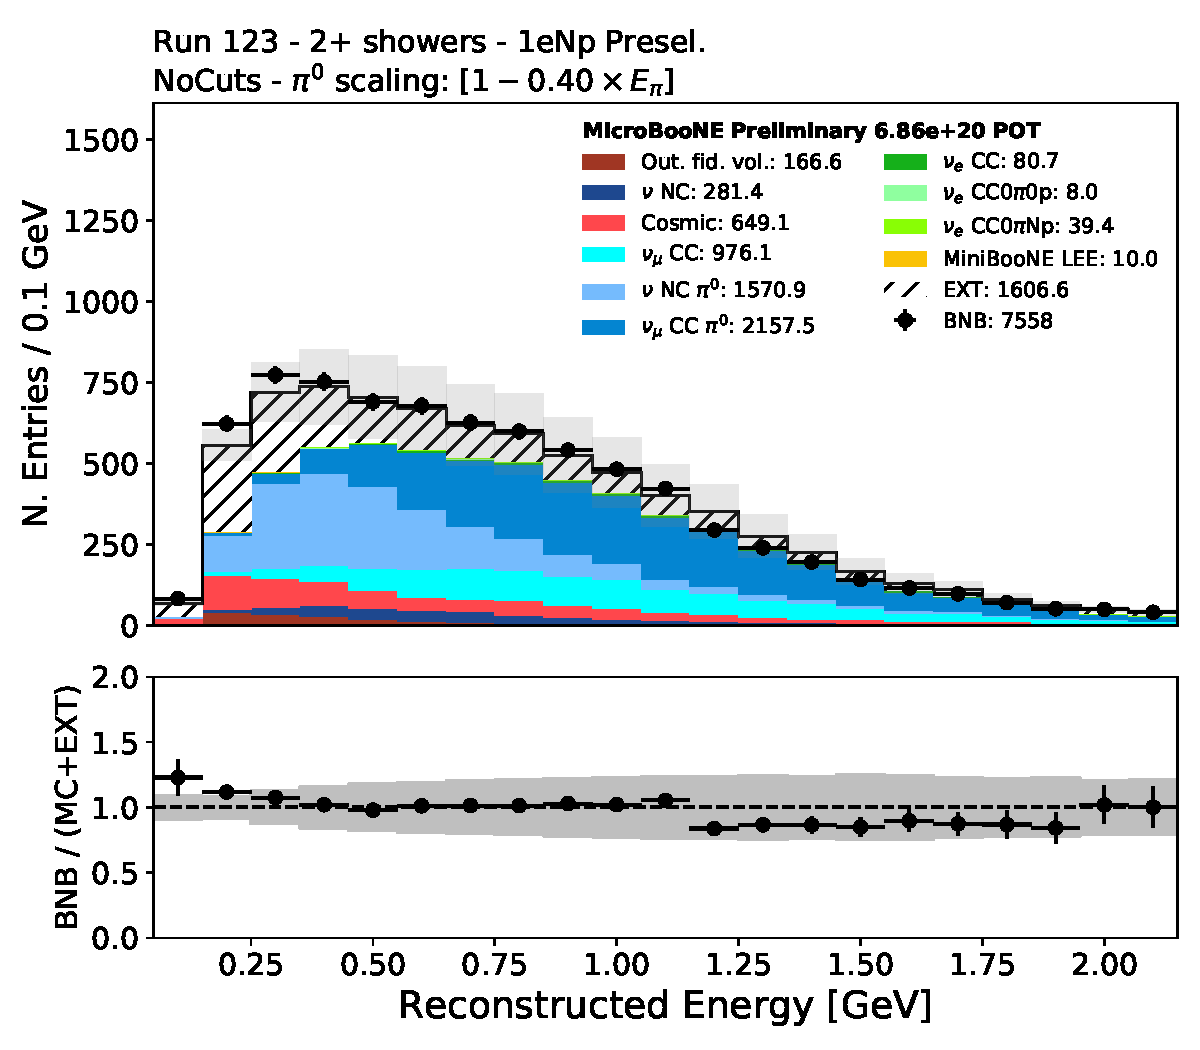
\includegraphics[width=0.5\textwidth]{Sidebands/Figures/1eNp/TwoShower/TwoPShr_NP_None_pi0e040/reco_e.pdf}
\caption{\label{fig:exampleplot}Example data/MC comparison to help illustrate the conventions and labels used throughout this document.}
\end{center}
\end{figure}

\subsection{Supporting Documentation for the Analysis}
The analysis presented in this Tech-Note relies on significant work from multiple fronts within the MicroBooNE Collaboration. Table~\ref{tab:documentation} tries to provide references for important technical documentation on which this analysis relies.

\begin{table}[H]
\centering
\setlength{\tabcolsep}{10pt}
\renewcommand{\arraystretch}{1.25}
 \begin{tabular}{| m {5 cm} | m {10 cm} |} 
 \hline
Reference & Description \\ \hline
\href{https://microboone.fnal.gov/wp-content/uploads/MICROBOONE-NOTE-1074-PUB.pdf}{NOTE-1074-PUB}, \href{https://microboone-docdb.fnal.gov/cgi-bin/private/ShowDocument?docid=27018}{DocDB 27018} & GENIE interaction model and model uncertainties \\ \hline
\href{https://microboone.fnal.gov/wp-content/uploads/MICROBOONE-NOTE-1075-PUB.pdf}{NOTE-1075-PUB}, \href{https://microboone-docdb.fnal.gov/cgi-bin/private/ShowDocument?docid=27009}{DocDB 27009} & Treatment of detector systematics \\ \hline
 \href{https://microboone-docdb.fnal.gov/cgi-bin/private/ShowDocument?docid=27042}{DocDB 27042} & Calorimetric reconstruction and calibrations \\ \hline
 \end{tabular}
 \caption{\label{tab:documentation}References for major contributions supporting this analysis.}
\end{table}
